% This is "aamas2012 .tex" August 2012 
% This file should be compiled with "aamas2012 .cls" 
% This example file demonstrates the use of the 'aamas2012 .cls'
% LaTeX2e document class file. It is for those submitting
% articles to AAMAS 2012  conference. This file is based on
% the sig-alternate.tex example file.
% The 'sig-alternate.cls' file of ACM will produce a similar-looking,
% albeit, 'tighter' paper resulting in, invariably, fewer pages.
% than the original style ACM style.
%
% ----------------------------------------------------------------------------------------------------------------
% This .tex file (and associated .cls ) produces:
%       1) The Permission Statement
%       2) The Conference (location) Info information
%       3) The Copyright Line with AAMAS data
%       4) NO page numbers
%
% as against the acm_proc_article-sp.cls file which
% DOES NOT produce 1) thru' 3) above.
%
% Using 'aamas2012 .cls' you don't have control
% from within the source .tex file, over both the CopyrightYear
% (defaulted to 200X) and the IFAAMAS Copyright Data
% (defaulted to X-XXXXX-XX-X/XX/XX).
% These information will be overwritten by fixed AAMAS 2012  information
% in the style files - it is NOT as you are used with ACM style files.
%
% ---------------------------------------------------------------------------------------------------------------
% This .tex source is an example which *does* use
% the .bib file (from which the .bbl file % is produced).
% REMEMBER HOWEVER: After having produced the .bbl file,
% and prior to final submission, you *NEED* to 'insert'
% your .bbl file into your source .tex file so as to provide
% ONE 'self-contained' source file.
%

% This is the document class for full camera ready papers and extended abstracts repsectively 

\documentclass{aamas2012}

% if you are using PDF LaTex and you cannot find a way for producing
% letter, the following explicit settings may help
 
\pdfpagewidth=8.5truein
\pdfpageheight=11truein

\begin{document}

% In the original styles from ACM, you would have needed to
% add meta-info here. This is not necessary for AAMAS 2012  as
% the complete copyright information is generated by the cls-files.


\title{A Formal Agent-based Framework to Model Virtual Worlds}

% AUTHORS


% For initial submission, do not give author names, but the
% tracking number, instead, as the review process is blind.

% You need the command \numberofauthors to handle the 'placement
% and alignment' of the authors beneath the title.
%
% For aesthetic reasons, we recommend 'three authors at a time'
% i.e. three 'name/affiliation blocks' be placed beneath the title.
%
% NOTE: You are NOT restricted in how many 'rows' of
% "name/affiliations" may appear. We just ask that you restrict
% the number of 'columns' to three.
%
% Because of the available 'opening page real-estate'
% we ask you to refrain from putting more than six authors
% (two rows with three columns) beneath the article title.
% More than six makes the first-page appear very cluttered indeed.
%
% Use the \alignauthor commands to handle the names
% and affiliations for an 'aesthetic maximum' of six authors.
% Add names, affiliations, addresses for
% the seventh etc. author(s) as the argument for the
% \additionalauthors command.
% These 'additional authors' will be output/set for you
% without further effort on your part as the last section in
% the body of your article BEFORE References or any Appendices.

%\numberofauthors{8} %  in this sample file, there are a *total*
% of EIGHT authors. SIX appear on the 'first-page' (for formatting
% reasons) and the remaining two appear in the \additionalauthors section.
%

\numberofauthors{5}

\author{
% You can go ahead and credit any number of authors here,
% e.g. one 'row of three' or two rows (consisting of one row of three
% and a second row of one, two or three).
%
% The command \alignauthor (no curly braces needed) should
% precede each author name, affiliation/snail-mail address and
% e-mail address. Additionally, tag each line of
% affiliation/address with \affaddr, and tag the
% e-mail address with \email.
% 1st. author
\alignauthor
Paper 209
%Ben Trovato\titlenote{Dr.~Trovato insisted his name be first.}\\
%       \affaddr{Institute for Clarity in Documentation}\\
%       \affaddr{1932 Wallamaloo Lane}\\
%       \affaddr{Wallamaloo, New Zealand}\\
%       \email{trovato@corporation.com}
% 2nd. author
%\alignauthor
%G.K.M. Tobin\titlenote{The secretary disavows any knowledge of this author's actions.}\\
%       \affaddr{Institute for Clarity in Documentation}\\
%       \affaddr{P.O. Box 1212}\\
%       \affaddr{Dublin, Ohio 43017-6221}\\
%       \email{webmaster@marysville-ohio.com}
% 3rd. author
%\alignauthor Lars Th{\o}rv{\"a}ld\titlenote{This author is the one who did all the really hard work.}\\
%       \affaddr{The Th{\o}rv{\"a}ld Group}\\
%       \affaddr{1 Th{\o}rv{\"a}ld Circle}\\
%       \affaddr{Hekla, Iceland}\\
%       \email{larst@affiliation.org}
}

%\and  % use '\and' if you need 'another row' of author names

% 4th. author
%\alignauthor Lawrence P. Leipuner\\
%       \affaddr{Brookhaven Laboratories}\\
%       \affaddr{Brookhaven National Lab}\\
%       \affaddr{P.O. Box 5000}\\
%       \email{lleipuner@researchlabs.org}

% 5th. author
%\alignauthor Sean Fogarty\\
%       \affaddr{NASA Ames Research Center}\\
%       \affaddr{Moffett Field}\\
%       \affaddr{California 94035}\\
%       \email{fogartys@amesres.org}

% 6th. author
%\alignauthor Charles Palmer\\
%       \affaddr{Palmer Research Laboratories}\\
%      \affaddr{8600 Datapoint Drive}\\
%       \affaddr{San Antonio, Texas 78229}\\
%       \email{cpalmer@prl.com}

%\and

%% 7th. author
%\alignauthor Lawrence P. Leipuner\\
%       \affaddr{Brookhaven Laboratories}\\
%       \affaddr{Brookhaven National Lab}\\
%       \affaddr{P.O. Box 5000}\\
%       \email{lleipuner@researchlabs.org}

%% 8th. author
%\alignauthor Sean Fogarty\\
%       \affaddr{NASA Ames Research Center}\\
%       \affaddr{Moffett Field}\\
%       \affaddr{California 94035}\\
%       \email{fogartys@amesres.org}

%% 9th. author
%\alignauthor Charles Palmer\\
%       \affaddr{Palmer Research Laboratories}\\
%       \affaddr{8600 Datapoint Drive}\\
%       \affaddr{San Antonio, Texas 78229}\\
%       \email{cpalmer@prl.com}

%}

%% There's nothing stopping you putting the seventh, eighth, etc.
%% author on the opening page (as the 'third row') but we ask,
%% for aesthetic reasons that you place these 'additional authors'
%% in the \additional authors block, viz.
%\additionalauthors{Additional authors: John Smith (The Th{\o}rv{\"a}ld Group,
%email: {\texttt{jsmith@affiliation.org}}) and Julius P.~Kumquat
%(The Kumquat Consortium, email: {\texttt{jpkumquat@consortium.net}}).}
%\date{30 July 1999}
%% Just remember to make sure that the TOTAL number of authors
%% is the number that will appear on the first page PLUS the
%% number that will appear in the \additionalauthors section.

\maketitle

\begin{abstract}
In the latest years, an important research has been focussed on the Multi-Agent Systems (MAS) and the Virtual Reality (VR) resulting in a spectacular progress. However, the potential of integrating both systems has not been exploited to its whole extent. Usually, the integration of MAS and RV are confined to endow the virtual system with Artificial Intelligence. 

This paper proposes a model based on grammars, the Virtual Worlds Generator (VWG), to develop complex virtual environments that integrates the MASs features. A virtual world is described as a set of dynamic and static elements. The static part is represented by a sequence of primitives and transformations and the dynamic elements by a series of agents. The agent activation and communication is achieved using events. The events are created by the event generators.

The grammar allows a descriptive language with a simple syntax, but the most interesting contribution is the semantics, defined by functions. The semantics functions for primitives and transformations allow the scene to be display in a graphics device. Nevertheless, the most important semantics functions are, perhaps, the so called evolution functions. The evolution functions allow the description of the activities of the agents, including AI algorithms, reactions to physical phenomena, or any other behavior.

To illustrate the use of VWG a practical example has been presented: a robot simulator which considers the main features of a typical robot. The result is a functional complete simulator.

As a result, the VWG is a reusable, integral and generic system, which can be easily increased, adapted, and improved. The description of the virtual scene is independent from its representation and the elements which it interacts with.
\end{abstract}

% Note that the category section should be completed after reference to the ACM Computing Classification Scheme available at
% http://www.acm.org/about/class/1998/.

\category{H.5.1}{Information Interfaces and Presentation}{Multimedia Information Systems}[Artificial, augmented, and virtual realities]

%A category including the fourth, optional field follows...
%\category{D.2.8}{Software Engineering}{Metrics}[complexity measures, performance measures]

%General terms should be selected from the following 16 terms: Algorithms, Management, Measurement, Documentation, Performance, Design, Economics, Reliability, Experimentation, Security, Human Factors, Standardization, Languages, Theory, Legal Aspects, Verification.

\terms{Design}

%Keywords are your own choice of terms you would like the paper to be indexed by.

\keywords{Multi-agent systems, Virtual Reality systems, grammatical models}

%___________________________________________________________________________
\section{Introduction
\label{sec:introduction}}
%___________________________________________________________________________

The growing influence of Multi-Agent Systems (MAS) in several fields of research (sociology,
economics, artificial intelligence, ecology, and so on) has led to a significant evolution in its
development. On the other hand, the spectacular progress of the Virtual Reality (VR) systems has contributed to present the information in a more immersive way using new forms of analysis \cite{Sherman2003}. Video games and the entertainment industry in general, have had a decisive influence on this
striking progress, that has arrived to the field of research \cite{Rhyne2000, Novak2007}. 

All these developments have opened up new challenges, among them the possibility of integrating MAS and VR systems. However, this potential has not been exploited to its whole extent. Whereas a VR system can be considered to be composed of three main modules (rendering system, Physics engine and Artificial Intelligence system), the integration of MAS and RV are usually confined to endow the system with Artificial Intelligence. 

There are many generic and specific work environments to develop MASs, but they seldom allow the definition of complete RV systems, such as advanced visual features or physics phenomena. For instance, in Sociology
\cite{Axelrod1997,Gilbert2008}, very specific solutions are used, generally
oriented to sociological studies, such as the movement of crowds
\cite{Ulicny2001,Reynolds2000}. In some cases, they use graphics to display statistics,
the density of agents within the environment or even simple animations of the movements of agents
\cite{Reynolds2000}. Netlog \cite{Wilensky1999} is a useful tool to study highly complex systems.
It has developed some graphical features, but the agents are just represented by Logo style triangles
just to allow the user to observe the movement of agents and the population density.
There are also some interesting works related to very specific aspects of graphical representation of characters in a virtual environment. Such are the cases of the use of agents to get an expressive gaze animation \cite{Thiebaux2009} or to control the movement of an skeleton-based human character \cite{Chiu2011}. All these examples deal with only few aspects of the graphical representation.

The applications of the MASs to endow a VR system with AI are much easier to be found. One of these systems
proposes an implementation of a virtual world where objects react to several gestures of the user
\cite{Maes1997}. The work of \cite{Wachsmuth1995} uses the concepts of perception of the MASs
applied to virtual reality, where the agents react interactively with the user.

In the area of the entertainment industry, some MASs applied to games can also be found. In this
case, the agents are usually called bots \cite{Khoo2002} and they are programmed as characters of
the game, with objectives, strategies and actions. Programming is done with a specific script
language for each game, so that characters cannot easily be transferred between games. These
systems are so successful that they are being used in research for some specific cases
\cite{Rhyne2000}.

An increasing variety of generic development environments with a similar philosophy are also
emerging: they implement the most important features of agents, i.e., perception of the world,
communication, reaction, and so on \cite{Gilbert2008}. Some examples are Repast \cite{North2005}
and MASON \cite{Luke2004}.

Agents are usually considered to have some generic characteristics that make them difficult to
model \cite{Gilbert2008}. Although there are some common strategies for implementing them, there is
a lack of a unified design pattern. As a consequence, some problems arise, such as the difficult
reproduction of the results provided by the MASs \cite{Axelrod1997}, the lack of a suitable visual
representation or the limited capabilities of interaction with the user and with the environment. Some new contributions try to describe multi-agent metamodels to standardize the design, simplify the implementation and integrate the agent frameworks into a single tool  \cite{Hahn2009}. MASs could take advantage of the wide research carried out in this fields to develop RV systems. In this context, some agent metamodels for virtual reality applications \cite{Querrec2011} have also been described. They cover some aspects of virtual reality, but always considering the AI modules and disregarding most aspects about the graphical representation and the physics.

As a conclusion, there is a variety of environments that implement the essential characteristics
of the MASs and, in some cases, they have some basic graphics functions. However, a model that
unifies the definition of MASs and the whole potential of RV has not been proposed.

This paper describes an integral model based on grammars to develop complex environments that take
advantage of the MASs and the RV systems features. This framework uses a descriptive language and discrete
events to specify all the features necessary to define an agent. It allows an easy interaction with
the user so that the initial conditions could be changed, the experiments can be reproduced and the
components of the scene are displayed in real time. It is also independent from the display and
interaction devices and it incorporates a Physics engine. Finally, the agents can be easily reused.

The following section provides a description of the proposed model. In section 3, a case of study
is proposed with the aim of showing the use of the whole system. Finally, some conclusions and
possible lines of future work are presented.

%___________________________________________________________________________
\section{Model for Virtual Worlds Generation
\label{sec:model}}
%___________________________________________________________________________

A virtual world can be described as a set of dynamic and static elements. The static part is made of a sequence of primitives and transformations defined in a representation system $G$, usually a geometric system. However, a primitive has not to be understood just as a draw primitive (e.g. a sphere) but also as any action on the representation system that may
be a visual action or not (e.g. a sound). A transformation is a modification on the primitive behavior. They will
affect the set of primitives inside their scope of application.

The agents are the dynamic elements and they are made of activities and an optional set of attributes that make up their internal state. Each activity is a process that is executed as a reaction to a given event. The agents can
have a geometrical representation, defined using primitives and transformations, depending on their
internal state.

An event executes an activity. Its generation is independent from the physical device. They provide
the different ways of communication in the MAS.

Those are the main elements of the proposed system. A formal mathematical model, Virtual World Generator (VWG) is presented, to precisely define these features. VWG is a grammatical model, where the whole scenes are represented with a string generated by a given grammar  $M$.

\begin{table}
\centering
\caption{Production rules for grammar M}
\label{tab:rulesGrammar}
\begin{tabular}{|ll|}
    \hline

    1. & \textbf{WORLD} $\rightarrow$ OBJECTS \\

    2. & \textbf{OBJECTS} $\rightarrow$ OBJECT $|$ OBJECT $\cdot$ OBJECTS \\

    3. & \textbf{OBJECT} $\rightarrow$ FIGURE $|$ TRANSFORMATION $|$ \\
            & $|$ AGENT \\

    4. & \textbf{AGENT} $\rightarrow$ $a_{st}^d$(OBJECTS), $a_{st}^d \in A_{ST}^D, d \subseteq D$, \\
           &$st \subseteq ST$ \\

    5. & \textbf{TRANSFORMATION} $\rightarrow t$(OBJECTS), $t \in T$ \\

    6. & \textbf{FIGURE} $\rightarrow$ $p^+$, $p \in P$ \\

    \hline
\end{tabular}
\end{table}

A string $w \in \Sigma^*$ is generated by the grammar $M$, if it can be
obtained starting with the initial symbol WORLD and using the given production rules  (table \ref{tab:rulesGrammar}), where 
$P$ is the set primitives, $T$ is the set of transformations,  $A_{ST}^D$ is the set of agents, that have some state from a set $ST$ and respond to some events of a set $D$. The symbols () indicate the scope and $\cdotp$ the concatenation of symbols. The
language $L(M)$ is the set of all the strings
which can be generated by this method, so:
$L(M) = \lbrace w \in \Sigma^* \ | \ \text{WORLD} \stackrel{*}{\rightarrow} w \rbrace$.
This grammar is a context-independent grammar (or a type-2 grammar, according to the Chomsky
hierarchy). Therefore, there is a procedure which verifies if a scene is correctly described.


%___________________________________________________________________________
\subsection{Semantics of the language $L(M)$
\label{sec:semantics}}

Apart from the language syntax, it is necessary to define the functionality of the strings, that is,
the semantics of the language. In our case, it is defined using a denotational method, which describes
the meaning of the string through mathematical functions.


%___________________________________________________________________________
\subsubsection{Semantic Functions for Primitives and Transformations (Rules 6 and 5)
\label{sec:rule6}}

Rule 6 defines the syntax of a figure as a sequence of primitives. Primitive's semantics is defined
as a function $\alpha: P \rightarrow G$. Each symbol in the set $P$ represents a primitive on a given geometric
system $G$. So, depending on the definition of the function $\alpha$ and on the geometric system $G$, the result
may be different. $G$ represents the actions which are run on a specific geometric system. An example
of geometric system are graphical libraries such as OpenGL or Direct3D. But, the function $\alpha$ has no
restrictions on the geometric system that can be applied to.

In Rule 5, the scope of a transformation is
limited by the symbols ``()''. Two functions are used to describe the semantics
of a transformation: $\beta: T \rightarrow G$ (it is carried out when the symbol ``('' is
processed), and $\delta: T \rightarrow G$ (it is carried out when the symbol ``)'' is found).
These two functions have the same features that the function $\alpha$, but they
are applied to the set of transformations $T$, using the same geometric system
$G$.

Given a string $w \in L(M)$, a new function $\varphi$ is defined to run a sequence of primitives $P$
and transformations $T$ in a geometric system $G$:


\begin{equation}
\begin{small}
    \varphi (w)=\left\{
    \begin{array}{ll}
        \alpha(w) & \mathit{if}  \ w \in P  \\

        \beta(t); \varphi(v); \delta(t) & \mathit{if} \  w = t(v) \wedge v \in L(M) \\
        & \ \ \ \ \ \ \ \ \ \wedge \ t \in T \\

        \varphi(s); \varphi(v)  & \mathit{if} \  w = s \cdotp v \wedge s, v \in L(M)
    \end{array}\right\}
\end{small}
\end{equation}



One of the most important features of this system is the independence from a specific graphics
system. The definition of the functions $\alpha$, $\beta$ and $\delta$ provides the differences in
behavior, encapsulating the implementation details. Therefore, the strings developed to define
virtual worlds may be reused in other systems.


%___________________________________________________________________________
\subsubsection{Semantic Function for Agents (Rule 4)
\label{sec:rule4}}

The semantics of agents is a function which defines its behavior or, in terms of VR systems based on frames, its evolution in time. This is why it is called
\textit{evolution function} $\lambda$ and is defined as:
$\lambda: L(M) \times E^D \rightarrow L(M)$, where $E^D$ is the set of events
for the device $D$ (considering these devices as
any software or hardware process that sends events). By applying the function
$\lambda(w, e^{f})$, $w \in L(M)$ is transformed into another string $u$,
which allows the system to evolve. It has a different expression depending on
its evolution, but the general expression is defined as:

\begin{small}
\begin{equation}
    \lambda (a_{st}^{d}(v),e^{f})=
    \left\{
    \begin{array}{ll}
        u \in L(M) & \mathit{if}  \ \ f = d \\
        a_{st}^{d}(v)  & \mathit{if}  \ \ f \neq d
    \end{array}\right\}
\end{equation}
\end{small}

The result $u$ of the function may contain or not the own agent, it can generate other
events for the next frame or change the state $st$ (i.e. the set of attributes) of the agent.
The function $\lambda$ can define a recursive algorithm, called
\textit{function of the system evolution} $\eta$. Given a set of
events $e^i, e^j, e^k,$ $\dots, e^n$ (denoted as $e^v$, where $v \in D^+$)
and a string $w$, it describes the evolution of the system at a given point
in time. This algorithm also uses the operator $\prod_{\forall f \in v}$ which concatenates
strings.

\begin{small}
\begin{equation}
    \eta (w, e^v) = \left\{
    \begin{array}{ll}
        w   & \mathit{if}  \ w \in P  \\

        t(\eta (v, e^v))    & \mathit{if}  \  w = t(v)  \\

        \underset{\forall f \in v}{ \prod }(\lambda (a_{st}^d (\eta
            (y, e^v)), e^f))    & \mathit{if}  \ w = a_{st}^d(y) \\

        \eta (s, e^v) \cdot \eta (t, e^v)   & \mathit{if} \  w = s \cdot t
    \end{array}\right\}
\end{equation}
\end{small}

For the visualization of an agent, it must be first converted into strings made up only
of primitives and transformations. This conversion is carried out by a special type of function $\lambda$
called \textit{visualization function} $\theta: L(M) \times E^V \rightarrow L(E)$, where
$V \subseteq D$ are events used to create different views of the system, $E^V$ are events
created in the visualization process, and $L(E)$
is a subset of the language $L(M)$, including only primitives and transformations, but no agents. This function is defined as:

\begin{small}
\begin{equation}
    \theta (a_{st}^d(v), e^f) =
    \left\{
    \begin{array}{ll}
        w \in L(E) & \ \ \mathit{if}  \ \ f = d \wedge d \in V \\
        \epsilon  & \ \ \mathit{if}  \ \ f \neq d
    \end{array}\right\}
\end{equation}
\end{small}

As with the function $\lambda$, an algorithm is defined for $\theta$. It returns a string $z \in
L(E)$, given a string $w \in L(M)$ and a set of events $e^v$, where $v \in V^+$ and $V \subseteq
D$. This function is called \textit{function of system visualization} $\pi$ and it is defined as:
$\pi: L(M) \times E^V \rightarrow L(E)$

\begin{small}
\begin{equation}
    \pi (w, e^v) = \left\{
    \begin{array}{ll}
        w   & \mathit{if}  \ w \in P^+  \\

        t(\pi (y, e^v))     & \mathit{if}  \  w = t(y)  \\

        \underset{\forall f \in v}{ \prod }(\theta (a_{st}^v (\pi
            (y, e^v)), e^f))    & \mathit{if}  \ w = a_{st}^v(y) \\

        \pi (s, e^v) \cdot \pi (t, e^v)    & \mathit{if}  \ w = s \cdot t
    \end{array}\right\}
\end{equation}
\end{small}



%___________________________________________________________________________
\subsubsection{Semantic Functions for OBJECT, OBJECTS and WORLD (Rules 1,
2 and 3)
\label{sec:rules123}}

The semantic function of WORLD is a recursive function
which breaks down the string of the WORLD and converts it into substrings of OBJECTS. Then, these
substrings are in turn broken down into substrings of OBJECT. And for each substring of OBJECT,
depending on the type of the object, the semantic function of agent, transformation or primitive is
run. 



%___________________________________________________________________________
\subsection{Activity and Events
\label{sec:activity_events}}

In MAS some mechanisms must be established to model its activities.
These activities are run by agents and are activated by events.
Not all activities are run when an event is received, they can also be run when certain
conditions are satisfied.
The following event definition is established: {\itshape
$e_c^d$ is defined as an event of type $d \in D$ with data $e$, which is carried out only when the
condition $c$ is fulfilled. When there is no condition, the event is
represented by $e^d$.} Events may include information identifying who sent the message. So, it provides a generic
communication system that can implement FIPA or KMQL \cite{Genesereth1995}.


%___________________________________________________________________________
\subsection{Input Devices and Event Generators
\label{sec:input_devices}}

It is necessary to establish the independence between the system and the input devices
that generate events (hardware or software). So, the events needed to make
the system respond to a set of input devices must be defined.
A new function called \textit{event generator} is defined as: {\itshape
Let $C^d(t)$ be a function which creates events of type $d$ at the time instant $t$,
where $d \in D$ and $D$ is the set of event types which can be generated by the system. }

It is important to note that event generators encapsulate the device-dependent code.
They also can model the communication processes that exist in a MAS (agent-agent and
agent-environment communication).

The process which obtains the events produced by input devices and their associated
generators is defined as follows: {\itshape
Let $C^*$ be the set of all the event generators which are associated with input
devices and $E(C^*, t)$ the function that collects all the events from all the generators, then:}


\begin{small}
\begin{equation}
     E(C^*, t) = \left\{
    \begin{array}{ll}
        e(z, C_i(t))   &  \mathit{if}  \ z = E(C^* - C_i, t) \\
        \epsilon   &  \mathit{if} \ C^* = \emptyset
    \end{array}\right\}
\end{equation}
\end{small}



where    $e(z, e^i) = \left\{
    \begin{array}{ll}
        z \cdot e^i   &   \mathit{if} \ e^i \notin z \\
        z    &   \mathit{if} \ e^i \in z
    \end{array}
    \right\}$



%___________________________________________________________________________
\subsection{System Algorithm
\label{sec:system_algorithm}}

Once all the elements involved in the model to manage a MAS have been defined, the algorithm which carries out the
entire system can be established, as shown in table \ref {tab:SysAlg}


\begin{table}
\centering
\caption{System algorithm}
\label {tab:SysAlg}
\begin{tabular}{|ll|}
    \hline
    1. & $w = w_o$; $t = 0$ \\
    2. & $e^* = E(G^*, t)$ \\
    3. & $e^v =$ events of $e^*$ where $v \in V^+$ \\
    4. & $e^u = e^* - e^v$ \\
    5. & $w_{next} = \eta(w, e^u)$ \\
    6. & $v =  \pi(w, e^v)$ \\
    7. & $g = \varphi(v)$ \\
    8. & $w = w_{next}; \ \ t = t + 1$ \\
    9. & If $w = \epsilon$ then go to 11 \\
    10. & Go to 2 \\
    11. & End \\
\hline
\end{tabular}
\end{table}

In table \ref {tab:SysAlg},  $w_o$ is the initial string of the system,  $e^*$ are all the events generated by the system in a frame $t$, $G^*$ = \{All the event generators which generate events of type $D$\}, $D$ = \{All the possible events in the system\}, $V$ = \{All the visual events\} where $V \subseteq D$, $e^v$ are all the events from visual devices, $e^u$ are all the events from non-visual devices, and $g$ is the output device.


Steps 2, 3 and 4 manage the system events. In step 5, the evolution algorithm is called to obtain the
string for the next frame. In steps 6 and 7, the visualization of the system is performed.
In step 8, the next iteration
is prepared. Step 9 checks if the current string satisfies the condition of completion: if the
following string is empty the algorithm ends (Step 11), otherwise the algorithm continues.

Step 5 and 6-7 can be parallelized because they do not share any data, so it would lead
to a faster system performance.


%___________________________________________________________________________
\section{Case Study
\label{sec:case_study}}
%___________________________________________________________________________

An example is proposed to illustrate the use of VWG. Specifically, a robot navigation simulator will be built.  To be as realistic as possible, most features of robots will be taken into consideration.
%___________________________________________________________________________
\subsection{Problem Description
\label{sec:description_problem}}

Let us consider a robot programmed to autonomously navigate in a known environment, and to transport objects from one place to another. It is equipped with several sensors that provide information about the environment. The information from the sensors can be used for different tasks. For instance, in our case, the inputs are the data from a range sensor, e.g. a laser, to detect obstacles and distances, and the image from a camera, to identify the objects and the places, using markers. As there are heterogeneous sensor inputs, some processes of sensor integration are needed for the robot to use the data of different nature to make decisions.

There is also a human supervisor controlling the robot tasks and giving some high level instructions, such as interrupt the current task, begin a new task or change the speed parameters.

A system like this can be modeled using a classical hybrid scheme (figure \ref{fig:hybrid}), based on the combination of a reactive system and a proactive system. The elements in the hybrid scheme and the elements of the VWG model can be easily related:

\begin{figure}
\centering
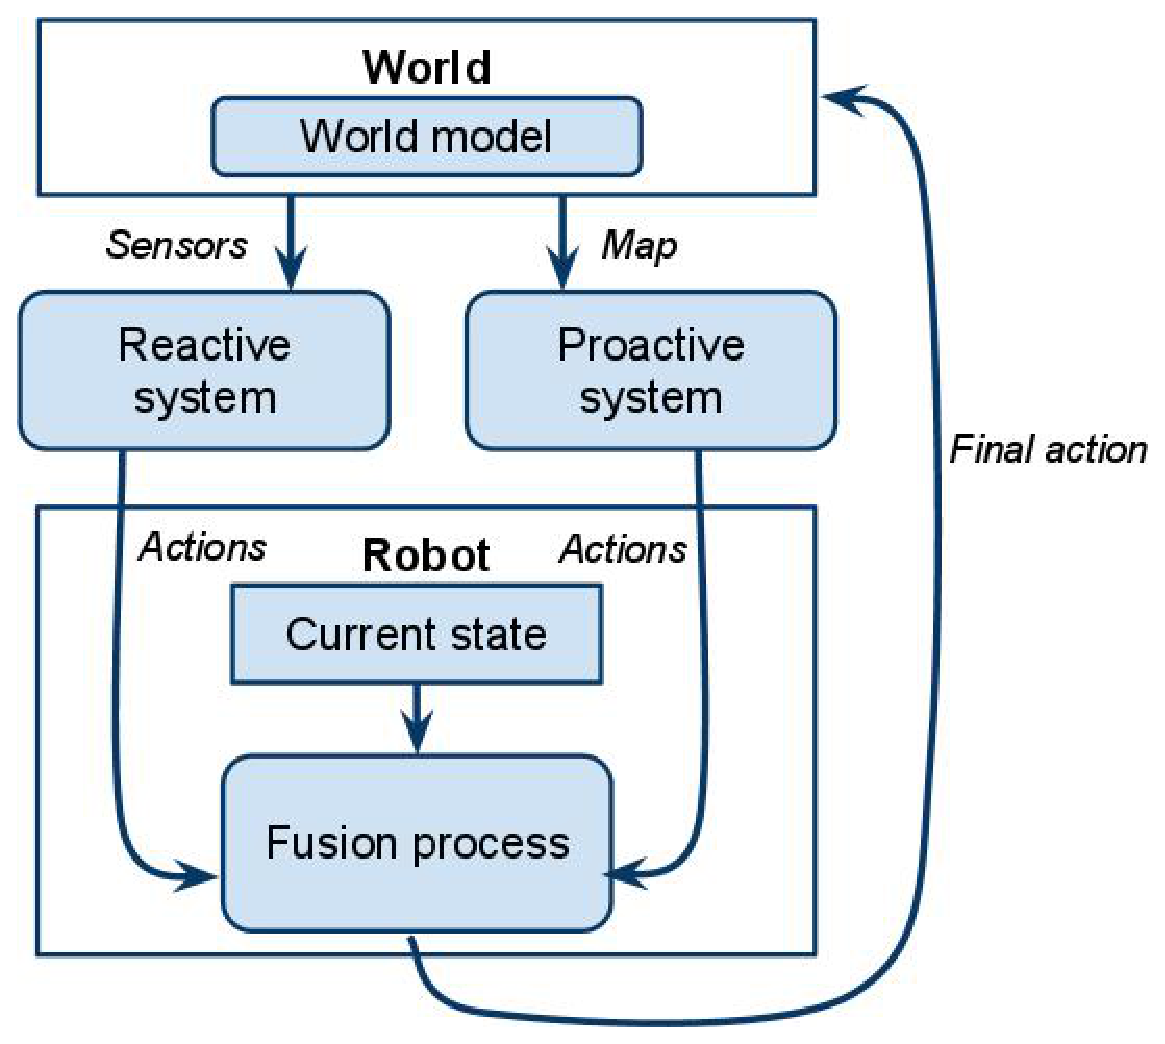
\epsfig{file=hybrid.jpg, width=6cm, height=6cm}
\caption{\label{fig:hybrid} Hybrid scheme for a robotic system.}
\end{figure}

\begin{itemize}
\item The world is the real environment.
\item The world model is a map, stored as an attribute of the agent robot.
\item The robot is the only agent in the system.
\item The reactive system is made of several generators, for the sensors and for the user's orders. 
\item The proactive system is the AI system of the robot, introduced in its evolution function.
\item The current state is the robot state (set of attributes).
\item The multisensorial fusion process is also introduced in the evolution function of the robot.
\item The final action is the result of the process of sensor integration and the final action carried out by the robot.
\end{itemize}

%___________________________________________________________________________
\subsection{Formalization}

When describing a system with VWG, the following aspects must be considered:
\begin{itemize}
\item The static displayable elements of the scene are described through the use of primitives, and the way to change their aspect are the transformations.
\item The dynamic elements are the agents.
\item For an agent to be displayable, there must be an associated primitive. 
\item Every aspect about the activities of the agents must be implemented in their evolution function, including AI algorithms, reactions to physical phenomena, and so on.
\item The events are the way to activate the actions of the agents and to communicate among them. The events can have themselves some attributes.
\item The agent attributes are the way to store all the information belonging to the agent.
\end{itemize}

%___________________________________________________________________________
\subsubsection{Primitives and transformations}

In our robotic system, only two primitives are needed, the map and the robot, which it is modified by two possible transformations: move and rotate (table \ref{tab:PrimTransf}). The primitives and the transformations will represent the operations carried out in the simulated robot, that is, the operations in the graphics system. The operations are performed by the semantic functions $\alpha$ for the primitives and $\beta$ and $\gamma$ for the transformations.

\begin{table}
\centering
\caption{Primitives and transformations of the robotic system}
\label {tab:PrimTransf}
\begin{tabular} {|l|l|l|}
\hline
Symbol & Meaning \\
\hline
\hline
$PMap$ & Draw the map\\ 
\hline
$PRobot$ & Draw the robot\\ 
\hline
$TMove_{<dist>}$ & Move a distance $dist$ \\
\hline
$TRotate_{<angle>}$ & Rotate an angle $angle$ \\
\hline
\end{tabular}
\end{table}

%___________________________________________________________________________
\subsubsection{Events and generators}

Each event is defined by its identifier and some attributes. They activate the changes on the agents, through their evolution functions. 
These events are produced by generators. There is a generator for each event type. In the robotic system, six generators are needed:
\begin{itemize}
\item gLaser: It generates an eLaser event when the laser detects an obstacle, by obtaining the laser data and processing them to find the possible obstacles.
\item gCamera: It generates an eCamera event when a marker is detected in the camera image. This generator is the responsible of obtaining the images, processing them and detect the markers. Markers are used to identify the rooms in the environment.
\item gDecide: It generates an eDecide event to report the system that a decision must be made. The system will use the accumulated information to activate the evolution function of the agents to make the correct decision, as it will be explained in the following sections.
\item gRepresent: It generates an eRepresent event to indicate the system to represent the robot actions in the current representation space. For our simulator, the operations will take place in the graphics system. In this case, it is similar to the usual 'redraw' event of a typical graphics system.
\item gObjective: It generates an eObjective event to set a new objective marker. This generator is connected to the user orders. Users can specify a new target room simply by selecting its associated marker.
\item gSpeed: It generates an eSpeed event when the user changes the robot speed.
\end{itemize}

The generators in our system and their associated events are shown in table \ref {tab:GenEvent}.

\begin{table*}
\centering
\caption{Generators and events of the robotic system}
\label {tab:GenEvent}
\begin{tabular} {|l|l|l|}
\hline
Generator and events & Event description & Associated data \\
\hline
\hline
$gLaser =  eLaser_{<dist,angle>}  \ if \ obstacle$ & The laser detects an obstacle & $dist, angle$:  obstacle position \\
\hline
$gCamera = eCamera_{<marker>} \ if \ marker$ & The camera detects a marker & $marker$: detected marker \\
\hline
$gDecide = eDecide \ each \ frame$ & The robot makes a decision & No data \\
\hline
$gRepresent = eRepresent \ each \ frame$ & The robot action is represented & No data \\
\hline
$gObjective = eObjective_{<marker>} \ if \ user \ order$ & The user sets the objective marker & $marker$: objective marker \\
\hline
$gSpeed = eSpeed_{<speed>} \ if \ user \ order$ & The user sets a new speed value & $speed$: robot speed \\
\hline
\end{tabular}
\end{table*}

An order relation must be defined to establish an execution priority among generators. In the robotic system, the order relation is: gLaser, gCamera, gSpeed, gObjective, gDecide, gRepresent. Therefore, events related with the acquisition of data have the highest priority, compared with the events of decision and execution.

%___________________________________________________________________________
\subsubsection{Agents}
The only agent in our robotic system is the robot which is defined as:

\begin{small}
\begin{displaymath}
ARobot^{eLaser, eCamera, eDecide, eRepresent, eObjective, eSpeed}_{<grid, row, column, angle, speed, objective, action>}
\end{displaymath}
\end{small}

where eLaser, eCamera, eDecide, eRepresent, eObjective and eSpeed are the events which the agent is prepared to respond to, and <grid, row, column, angle, speed, objective, action> are the attributes that make up its state, whose meanings are:

\begin{itemize}
\item grid: is a matrix of $mxn$ cells, representing the environment where the robot moves in. Each cell stores the registered data obtained from the sensors, that is, the detected obstacles and markers.
\item row, column: position occupied by the robot in the grid.
\item angle: robot orientation, defined by an angle.
\item speed: robot speed, defined by a numerical value.
\item objective: objective room, represented by its marker.
\item action: string of primitives and transformations which indicates the next command to be executed.
\end{itemize}

To simplify, in the following equations this agent will be referred as $ARobot^{E}_{<g, r, c, ang, s, o, act>}$.

The evolution function is, probably, the most important element in the system, as it defines the way the robot behaves in the environment. Let $e$ be an event that is received by the agent, the evolution function is defined as:

\begin{small}

$ \lambda (ARobot^{E}_{<g, r, c, ang, s, o, act>}, e)= $

\begin{displaymath}
    \left\{
    \begin{array}{ll}
        ARobot^{E}_{<g', r, c, ang, s, o, act>} & \mathit{if}  \  e = eLaser_{<dist,angle>} \\ \\
      ARobot^{E}_{<g', r, c, ang, s,  o, act>} & \mathit{if}  \  e = eCamera_{<marker>} \\ \\
       ARobot^{E}_{<g, r', c', ang', s, o, act'>} & \mathit{if}  \  e = eDecide \\ \\
         \alpha(ARobot^{E}_{<g, r, c, ang, s, o, act>}) & \mathit{if}  \ e = eRepresent \\ \\
          ARobot^{E}_{<g, r, c, ang, s, o', act>} & \mathit{if}  \ e = eObjective_{<marker>} \\ \\
          ARobot^{E}_{<g, r, c, ang, s', o, act>} & \mathit{if}  \ e = eSpeed_{<speed>} \\ \\
           ARobot^{E}_{<g, r, c, ang, s, o, act>} & otherwise
    \end{array}\right\}
\end{displaymath}
\end{small}

where the symbol apostrophe (') on an attribute indicates that it is changed. The changes in the attributes are:

\begin{itemize}
\item If $e=eLaser_{<dist,angle>}$, the grid ($g$) must be updated to indicate that an obstacle has been detected. The cell to mark is the one in position $(r+dist\ \cos(ang+angle), c+dist \ \sin(ang+angle))$.
\item if $e = eCamera_{<marker>}$ the grid ($g$) must be updated to indicate that a marker has been detected. The cell to mark is the one in position $(r+dist \ \cos(ang), c+dist \ \sin(ang))$.
\item if $e = eDecide$, the current position and orientation of the robot row ($r$), column ($c$) and angle ($ang$), must be updated, as well as the actions to be executed. This function is very important, as it provides the behavior of the robot. In the section \ref{sec:CaseEvolFunction}, the way to introduce intelligent behaviors and the Physics engine will be shown.
\item if $e = eRepresent$, the robot must be executed in the representation space, through the use of the $\alpha$ function.
\item if $e = eObjective_{<marker>}$, a new objective has been set by the user, so the objective ($o$) must be changed to the new one ($marker$).
\item if $e = eSpeed{<speed>}$, a new value for the speed has been set by the user, so the speed ($s$) must be updated.
\end{itemize}
In any other case, the agent must remain unchanged.

%___________________________________________________________________________
\subsubsection{Initial string}

The initial string in our system defines its initial state. It is the string 

\begin{small}
\begin{displaymath}
PMap \cdotp ARobot^{eLaser, eCamera, eDecide, eRepresent, eObjective, eSpeed}_{<grid, row, column, angle, 0, \epsilon, \epsilon>}
\end{displaymath}
\end{small}

 where the attribute grid is initialized to a set of empty cells, the attributes row, column and angle are initialized to the initial position and orientation of the robot, the initial speed is 0, and the objective and the actions are defined as empty.

%___________________________________________________________________________
\subsubsection{Evolution function
\label{sec:CaseEvolFunction}}

As it was stated in section 3.2.3, the evolution function is the way of introducing behaviors in an agent. The key is implementing the AI algorithms and the Physics engine into this function, given that all the needed elements are known. For instance, in the robot simulator, the intelligent actions are triggered when an $eDecide$ event is received. The current grid is known, since it has been built as the $eLaser$ and $eCamera$ events have been received, the current position and orientation of the agent is also known, the speed has been defined by the user, and the objective has also been fixed by the $eObjective$ event. The implemented algorithm must decide the new position and orientation, and the next action to do. The specific algorithm to make this decision is up to the user, since the aim of this work is not to obtain the best AI algorithm to achieve the goal. In our case, to prove that any intelligent behavior can be introduced by just changing the evolution function, two simple decision algorithms have been chosen to decide how the robot should move in the world. The first algorithm is the simplest one: make decisions randomly to find the target position. The second algorithm is the A* algorithm  \cite{Luo2010}, considering the Euclidean distance to the goal as the weights. If there is an obstacle the distance is defined as infinite. 

%___________________________________________________________________________
\subsection{Features of the system}

One of the main features of our model is that the system definition is independent from the input devices. For instance, in our original system, a laser range sensor was used to detect obstacles. However, a different sensor, such as a Kinect device, may be introduced. To add this new device,  just a new event generator must be defined,  to create events of the same type that the ones generated by the laser generator. That is, it provides the same information: the angle and the distance to the obstacle. The new device is then introduced with no other modification in the system. The Kinect is then used to replace the laser device or to obtain redundant information for the detection of obstacles.

Maybe, the most important achievement in the proposed model is the fact that the description for the simulation can be used with a different representation system of even with the real robot with minor changes. In fact, the system definition, i.e. the string representing the system, remains exactly the same. To achieve this goal, only the generator for the execution of the robot commands and the visualization functions must be changed. The commands are transparently executed no matter whether the robot is real or simulated in any representation system, just using the appropriate generator. As a result, the navigation would be exactly the same for the simulated robot and for the real one, if there were not odometry errors. An example of this feature is shown in figures \ref{fig:map2D} and \ref{fig:map3D}, with two different representations, in 2D with sprites and in 3D with OpenGL.

\begin{figure}
\centering
\epsfig{file=map2D.jpg, width=6cm, height=6cm}
\caption{\label{fig:map2D} Sprite view in 2D.}
\end{figure}

The proposed model is, by definition, easily extensible, too. The updating of the definition string supposes the extension of the model and the addition of new features. Moreover, most elements can be reused in new definition strings to obtain new behaviors with little effort. In our case, new instances of the agent symbols (representing robots) have been added to the definition string to extend the system in an almost immediate way. 

 A good way to improve the simulation is introducing some odometry errors in the motors and in the sensor signals, accordingly with the features of the real robot.

\begin{figure}
\centering
\epsfig{file=map3D.jpg, width=6cm, height=6cm}
\caption{\label{fig:map3D} OpenGL view in 3D.}
\end{figure}


%___________________________________________________________________________
\section{Conclusions and Future Work
\label{sec:conclusions}}
%___________________________________________________________________________


A new agent-based framework to model virtual scenes, the Virtual Worlds Generator, has been presented. The major goal of this system is to take advantage of the MASs features to model a whole VR system, including the AI modules, the Physics engine and the graphics system. The proposed model uses a context-free grammar.

The key of the proposed model is the evolution function: it allows the definition of the behaviour of the agents, e.g.  the evolution of the elements in time. This way, the virtual world can be modeled as a set of static and dynamic elements, that have a visual representation, evolve during the execution and behave in accordance to AI algorithms or reacting to Physics phenomena.

The presented model separates the hardware-dependent implementation of the interaction devices from the description of the scene. This separation is made by event generators, that create a layer between the hardware and the representation of the system. The generators are mathematical models used to transform device actions, both visual and input devices, into more general actions. The
system must be able to identify these general actions regardless of the origin of the action. It is
achieved using abstraction. As a consequence of these features, the different elements of the system can be easily reused.

Using the proposed system, the Physics phenomena can be easily defined. It is achieved by setting up different types of event generators. Depending on the
physical features of the device, it activates the activity of the needed agent to react to that
physical process. For example, if an agent has to react to collisions, the event generator of this
type calculates the collisions between elements by extracting the scene geometry from the graphics
engine (it uses the implementation of the functions $\alpha$, $\beta$ and $\delta$ to calculate the
bounding box of the elements). Then, it generates the events needed to react to such collisions.
This event generator could be implemented with hardware if the system allows it.

The AI engine can also be implemented in the evolution function of the agents. Agents use these
functions to make decisions according to their current status. Moreover, events trigger activities
which can change the status and the behaviour of agents. The integration between the Physics engine
and the AI engine is guaranteed because both engines are connected by events.

Finally the framework has proven its usefulness, since a complete VR system has been built using it. The resulting model has shown to be expressive enough to model all the features of a functional robot simulator, such as the control of a mobile robot, the navigation in a given environment, and the process of a set of several inputs from different types of sensors. Moreover, the system can be directly implemented on a real robot, just making minor changes. In fact, the only thing to do is changing the representation space, using the real robot instead of the OpenGL environment. It would be achieved by redefining functions $\alpha$, $\beta$ and $\delta$ to make actions on the real robot.

The model presented in this work is currently under development. It is pretended to continue
developing several issues. One point to investigate is the optimization of the algorithm and its parallelization. The definition of the system through
strings facilitates the possibility of parallel algorithms. From another point of view, strings
represent the states of the system and its evolution. This evolution may change through mutations,
so different evolutive solutions may be conceived to design new systems. We also consider the
possibility of a new type of events which are activated with a certain probability. For example, if
an agent is defined as $a^{d,h}$ and it receives the event $e^d$, then the function associated with
this event will be carried out only with a certain probability.

In conclusion, the main aim has been to design a reusable, integral and generic system, which can be easily
increased, adapted, and improved. It is also important that the core of the system (the evolution
in time) is independent from its representation and the elements which it interacts with.

%\end{document}

%
% The following two commands are all you need in the
% initial runs of your .tex file to
% produce the bibliography for the citations in your paper.
\bibliographystyle{abbrv}
\bibliography{biblioVWG}  
% sigproc.bib is the name of the Bibliography in this case
% You must have a proper ".bib" file
%  and remember to run:
% latex bibtex latex latex
% to resolve all references
%
% ACM needs 'a single self-contained file'!
%
%APPENDICES are optional
%\balancecolumns
\end{document}
